\documentclass{article}
\usepackage[utf8]{inputenc}
\usepackage{graphicx}
\title{Mini Courses Portal}
\author{Vinay Kr. Singh(201402035) and Aman Varshney(201402188)}
\date{May 2015}

\begin{document}

\maketitle

\section{Brief Description of the Mini Courses Portal}

\large{Mini Courses Portal is designed to provide students a site where they can conquer and learn different courses.It gives them a platformto know about different subjects and clear their doubts with the threads available to them at the portal.They can subscribe and unsubscribe courses from their account.Add courses will give them an option to add course from the entire list of courses available.Only the admin(here manager) can add new courses to the data base.As taking into consideration that always courses are added according to the need of users.}


\section{Features Implemented}

\subsection{Login, Register, Forgot password}

\large{It gives a formal login option to all the users.If it would be an admin(here manager) he/she will have privilege to add new courses to the data base. Only managers account have a menu bar tab of 'manage',rest other users will have only three tabs in menu bar 1.Home ->which shows the cources you have subscribed.
2.Add Courses->gives you list of al courses and an option to subscribe them.
3.Remove Courses->gives a list of subscribed courses to unsubscribe.
if its a new user he/she needs to register first.And we have already fixed one user as a manager.}
\subsection{The layout of the pages}

\large{In this portal we have used many diffeent layouts which gives the app a WOW factor. Many similar layouts are available at web2py layouts site, we have modified the layouts to be used as per our requirement.}

\subsection{Adding Courses to Database}
\large{The admin(here manager) can add new courses to the database anytime he wishes by filling in the details.This feature is priviledged and can be accessed only by the admin(here manager).}

\subsection{Threads at the courses portal}
\large{Any user can post their doubts queries ans suggestions to the admin(here manager) anytime.Any user Admin or normal user can see those yhreads by clicking on the topics which are courses specific.
User can share its own topic thread too.}

\section{Features that need more work}
\subsection{Email sending to all the users}
\large{Whenever the admin(here manager) adds a new couse to database an e-mail should be sent to all the registered users.the mail shold contain full detail of the course like Course Name,Faculty Name,Short description,a mini image of course. }

\section{Schema of tables used}
\large{Table with name 'Courses' contains detail about Courses,'students' contains the registered users and 'posts' the  threads detail.}  

\newpage
\section{UI Screenshots}

\begin{figure}[ht!]
\centering
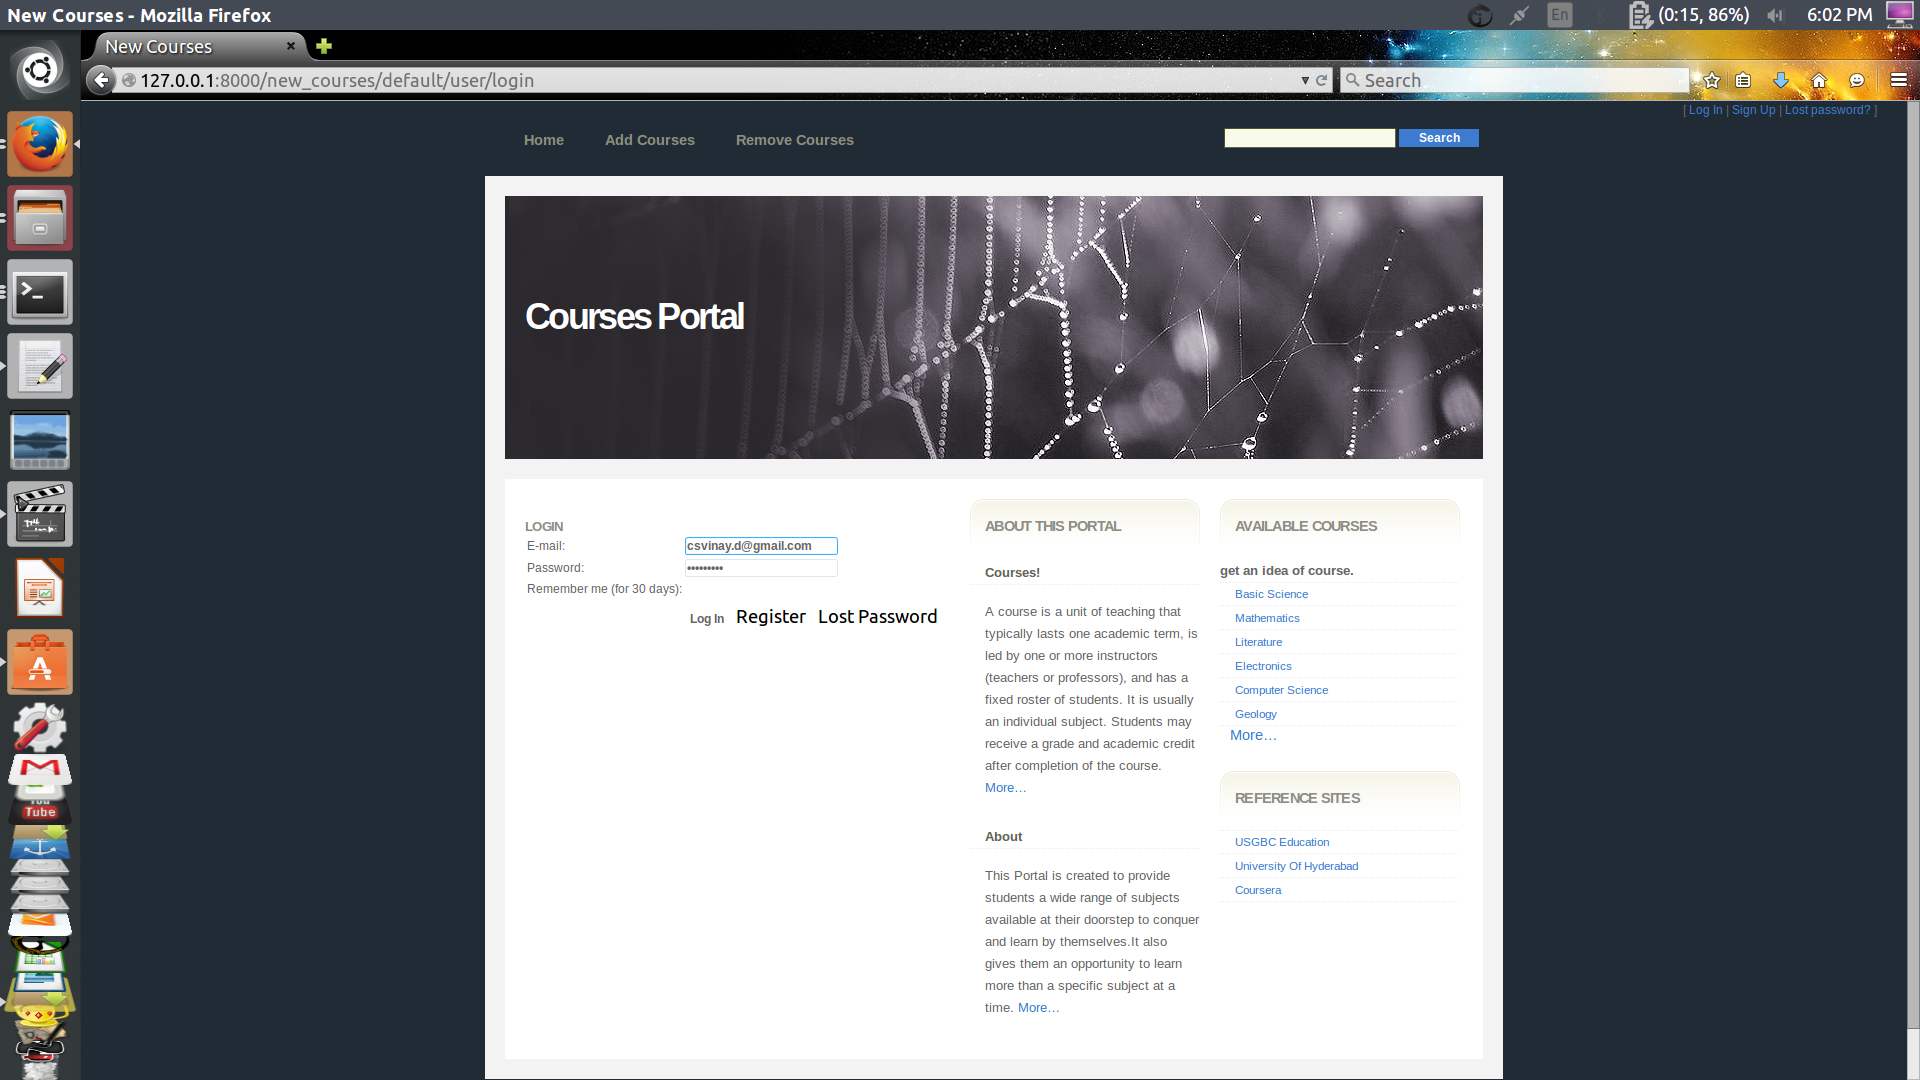
\includegraphics[width=110mm]{login.png}
\caption{Login page}
\end{figure}
\begin{figure}[ht!]
\centering
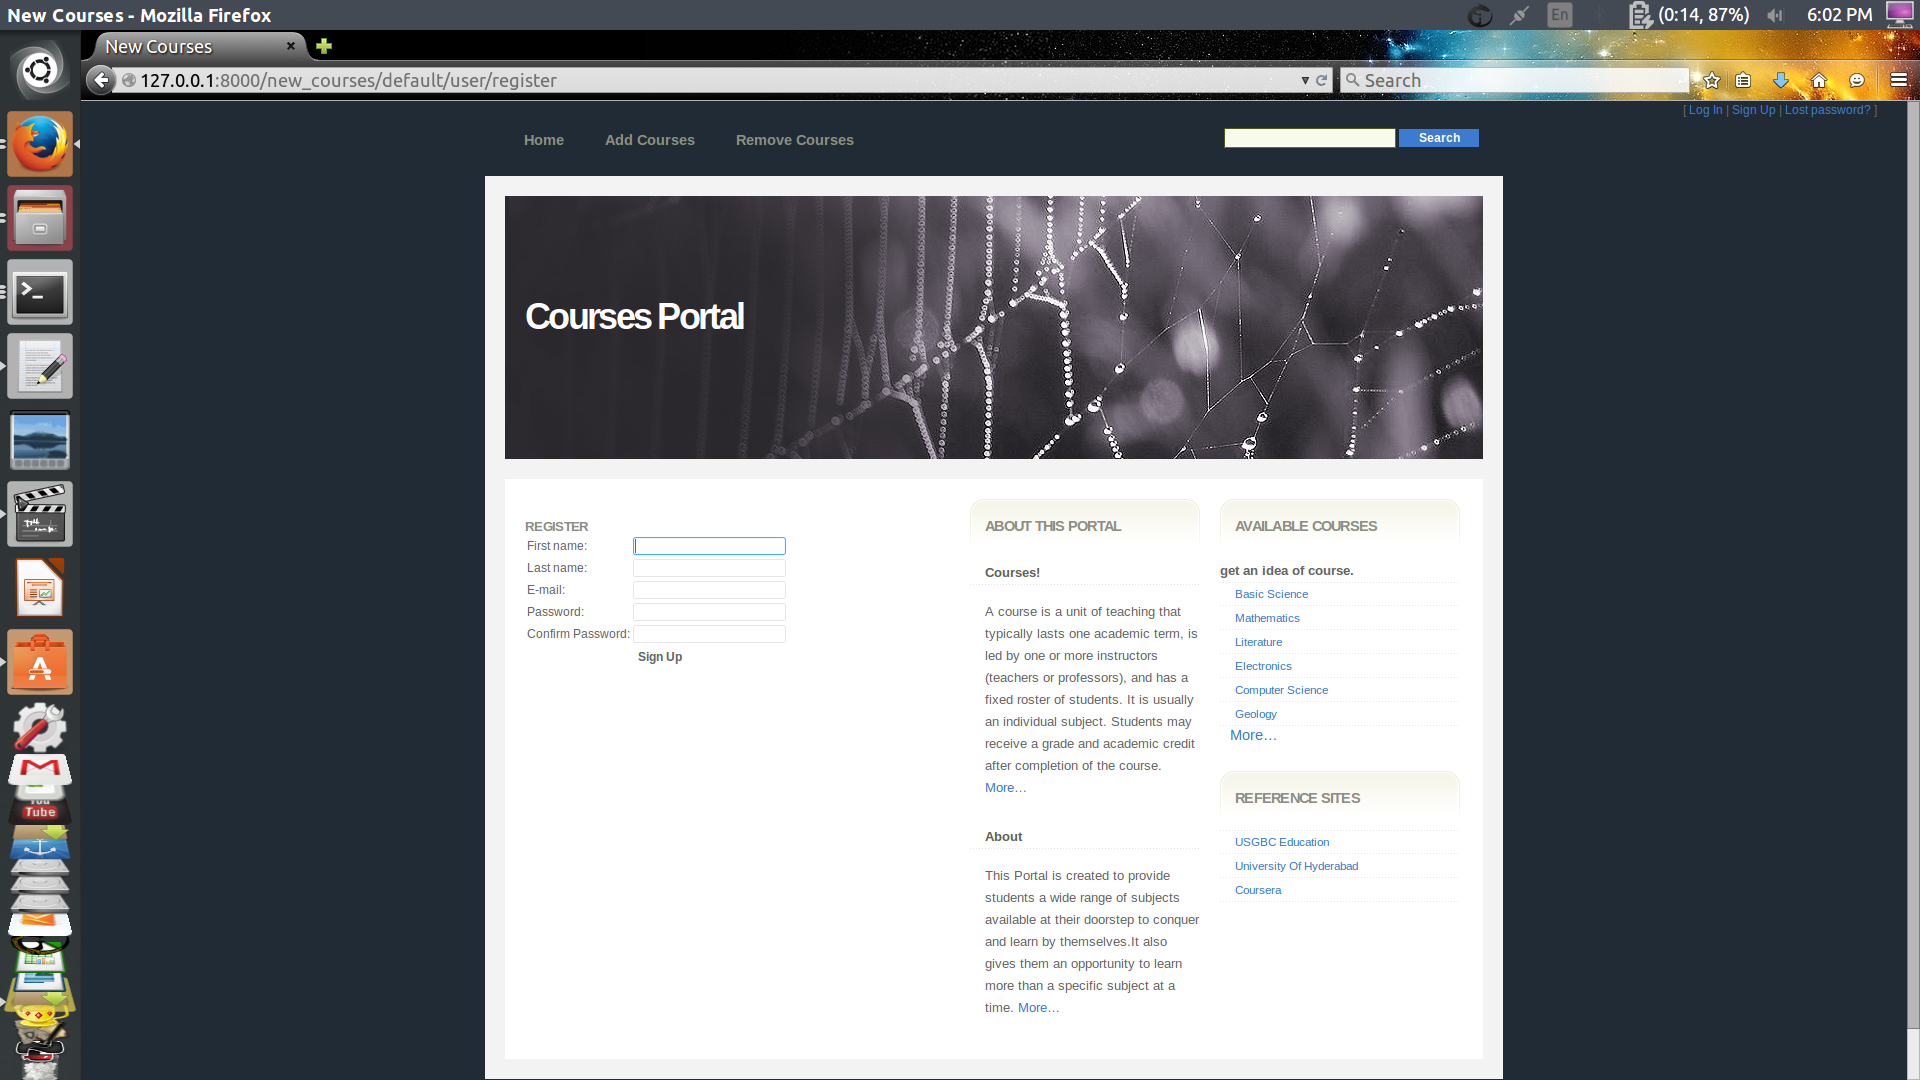
\includegraphics[width=110mm]{register.png}
\caption{register new user}
\end{figure}
\begin{figure}[ht!]
\centering
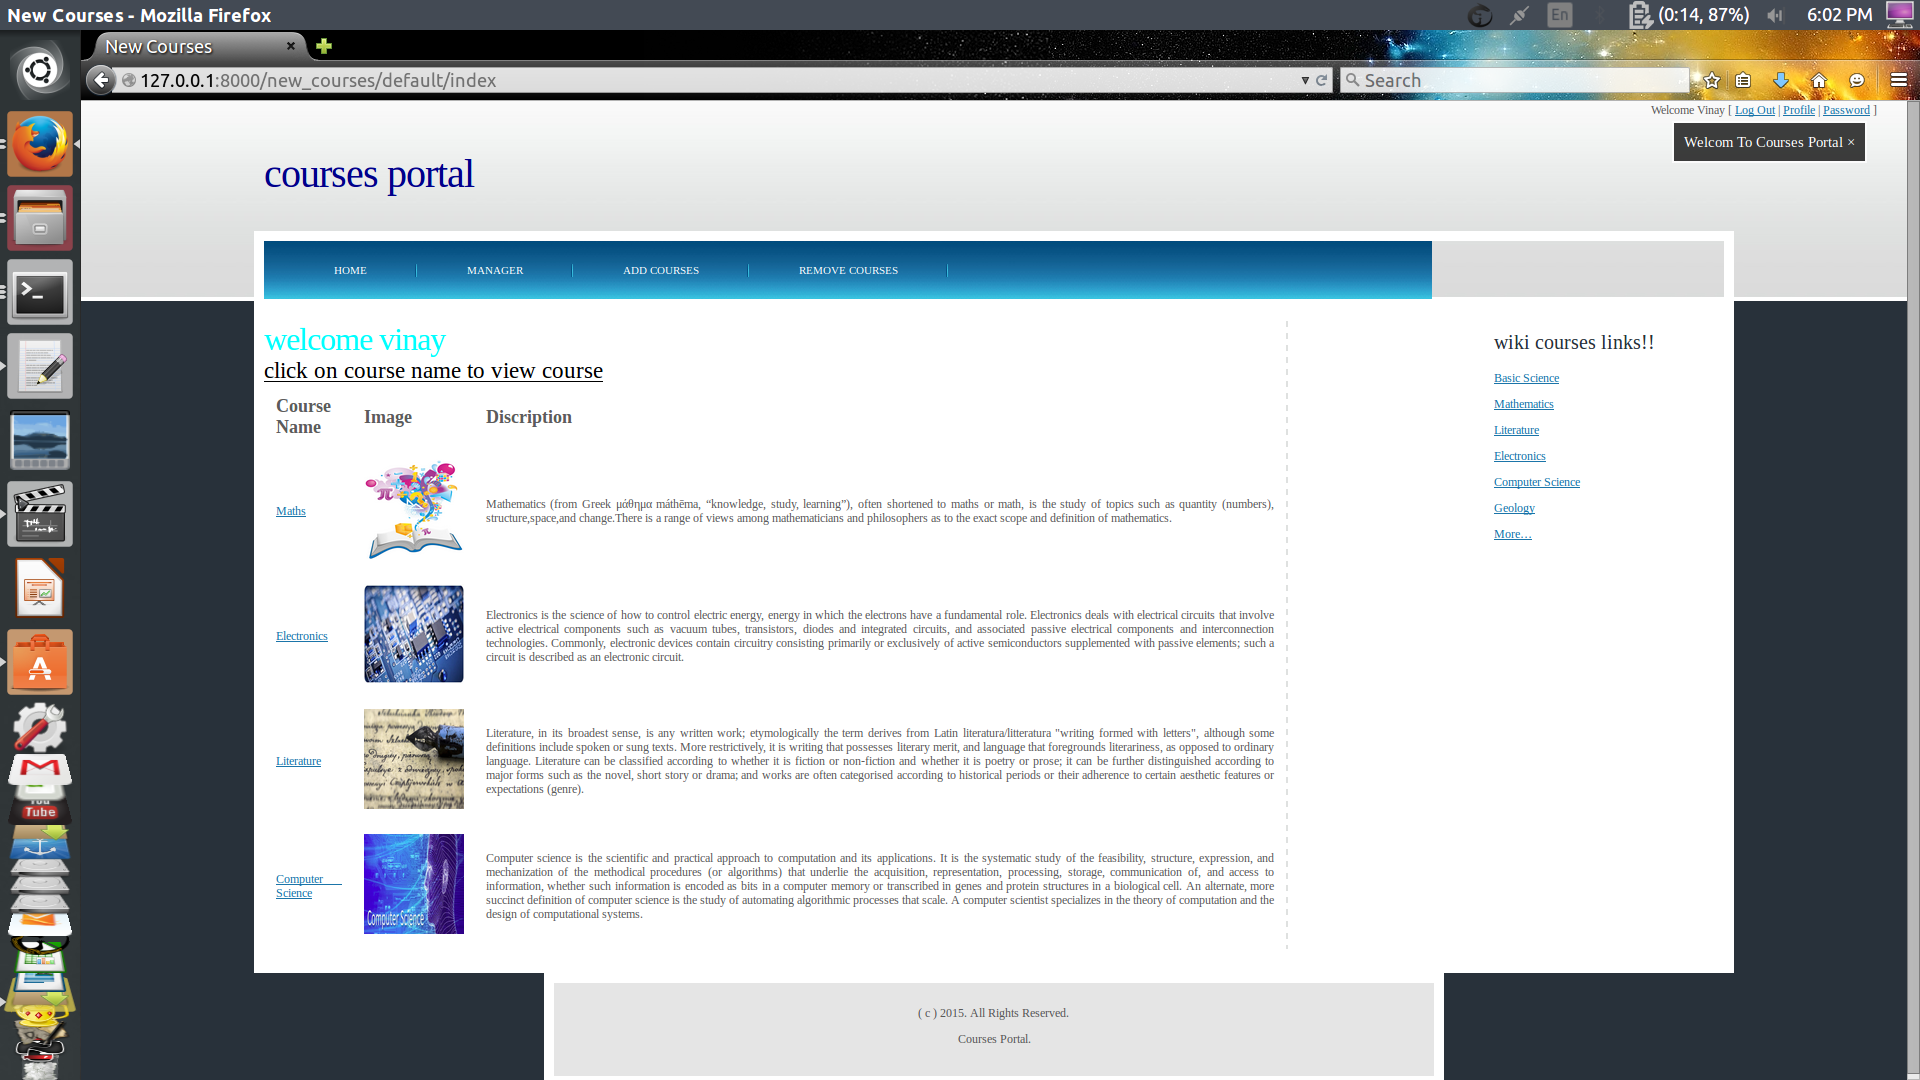
\includegraphics[width=110mm]{home.png}
\caption{Admins home}
\end{figure}
\begin{figure}[ht!]
\centering
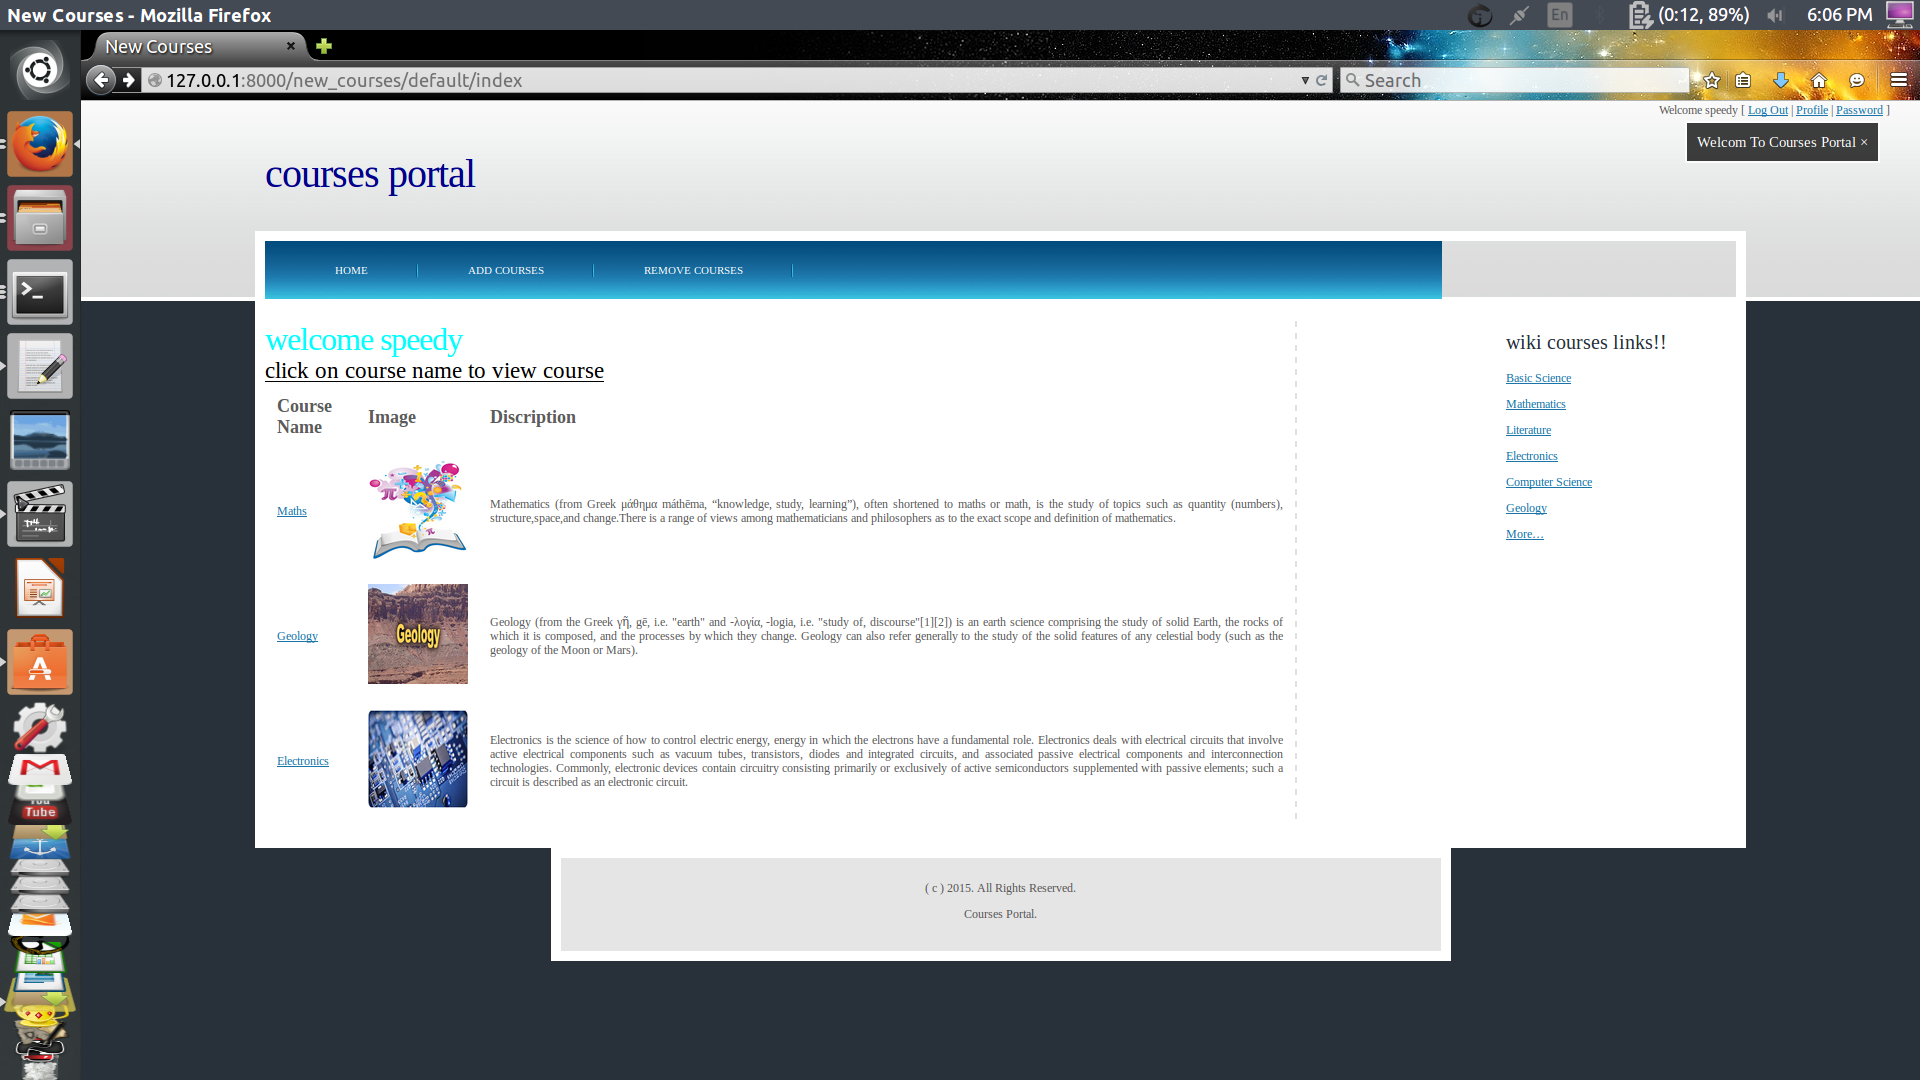
\includegraphics[width=110mm]{User_home.png}
\caption{Normal user's home}
\end{figure}
\begin{figure}[ht!]
\centering
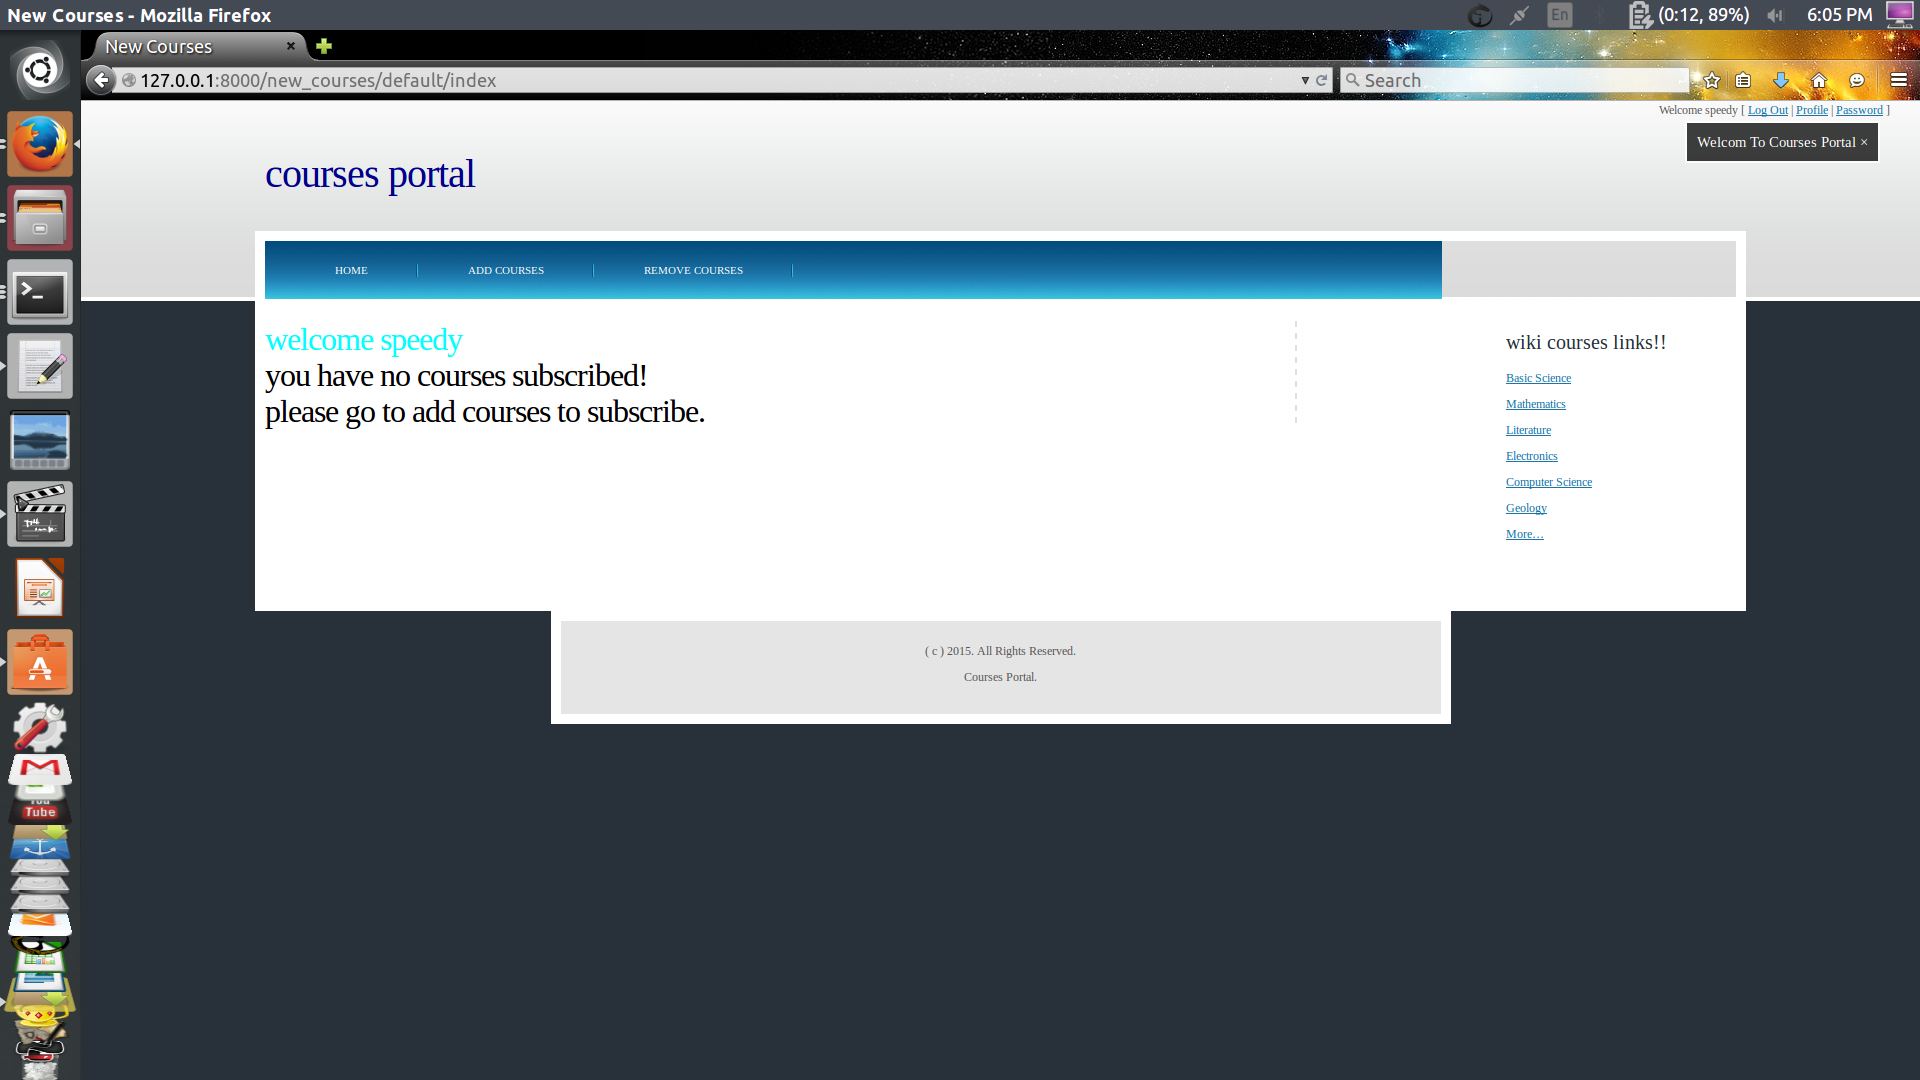
\includegraphics[width=110mm]{new_user.png}
\caption{New user's home}
\end{figure}
\begin{figure}[ht!]
\centering
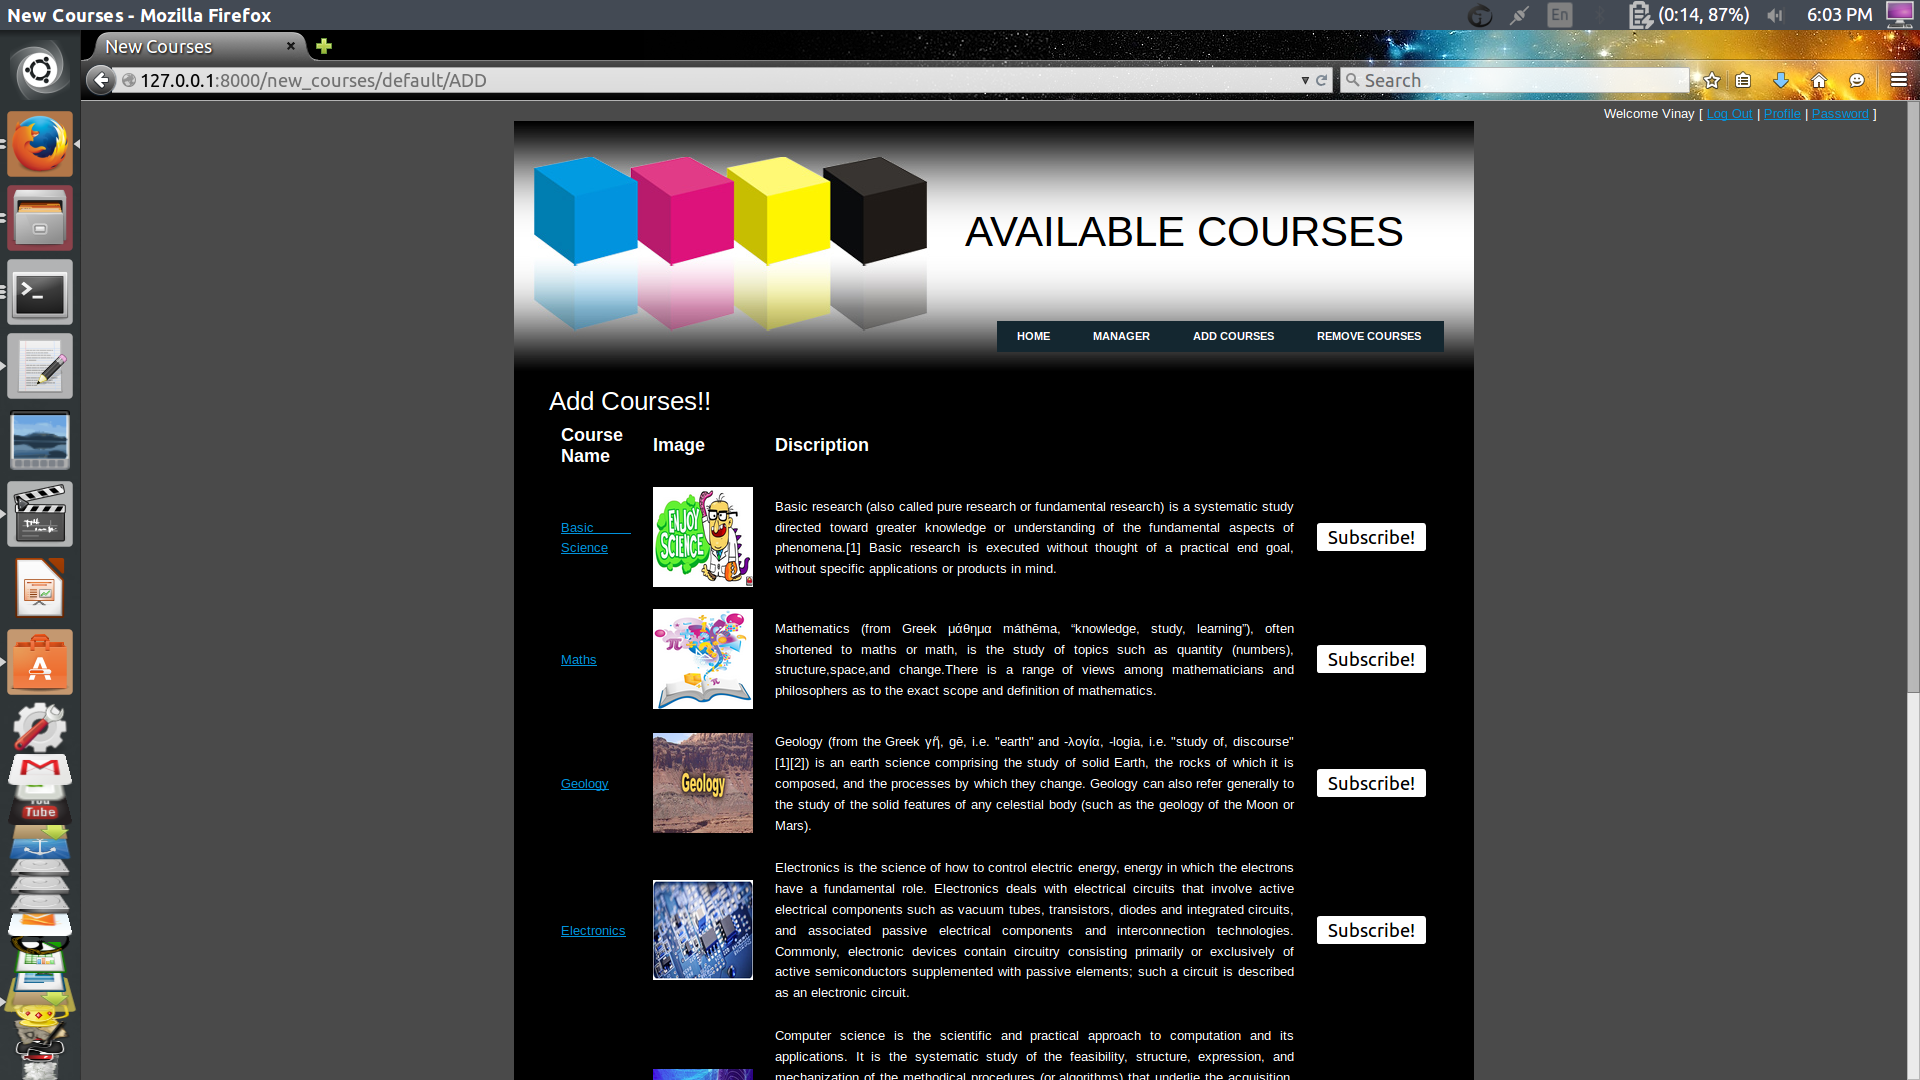
\includegraphics[width=110mm]{ADD.png}
\caption{Add new course}
\end{figure}
\begin{figure}[ht!]
\centering
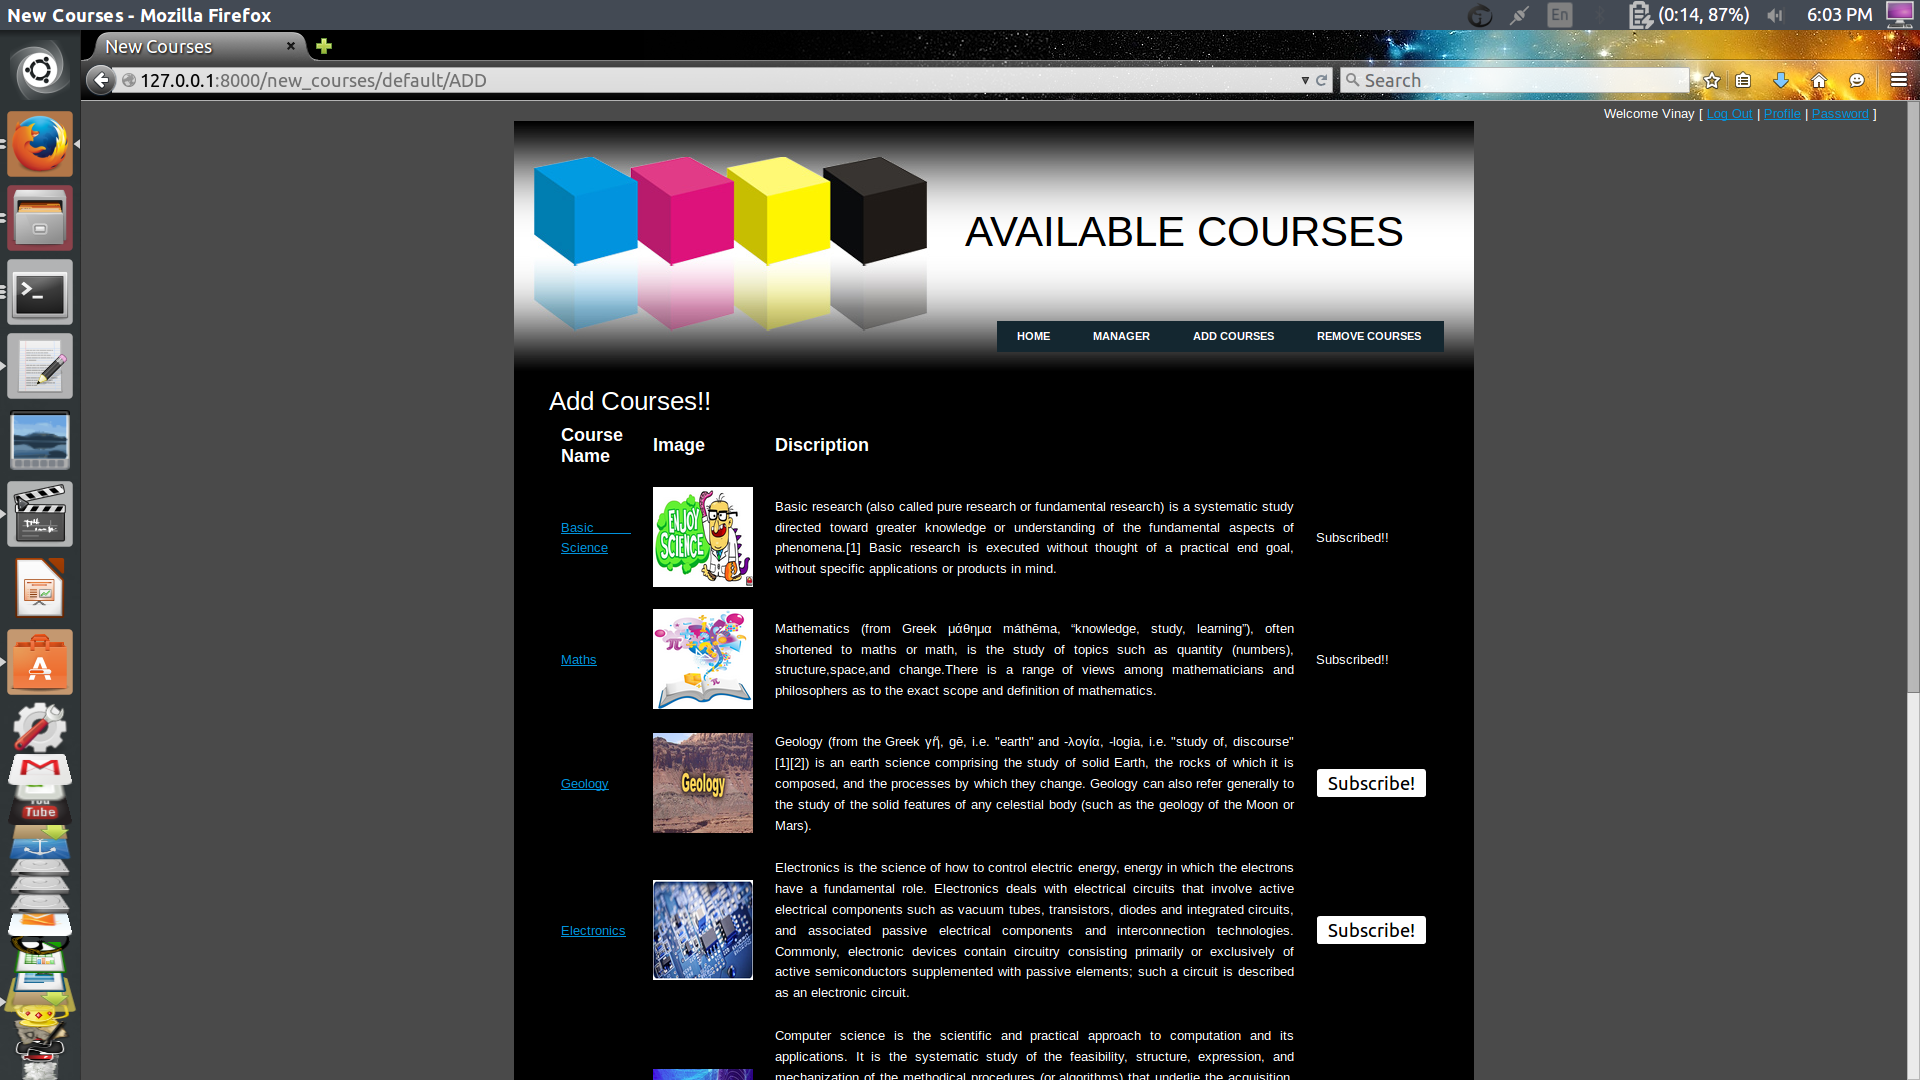
\includegraphics[width=110mm]{added.png}
\caption{Added new course}
\end{figure}
\begin{figure}[ht!]
\centering
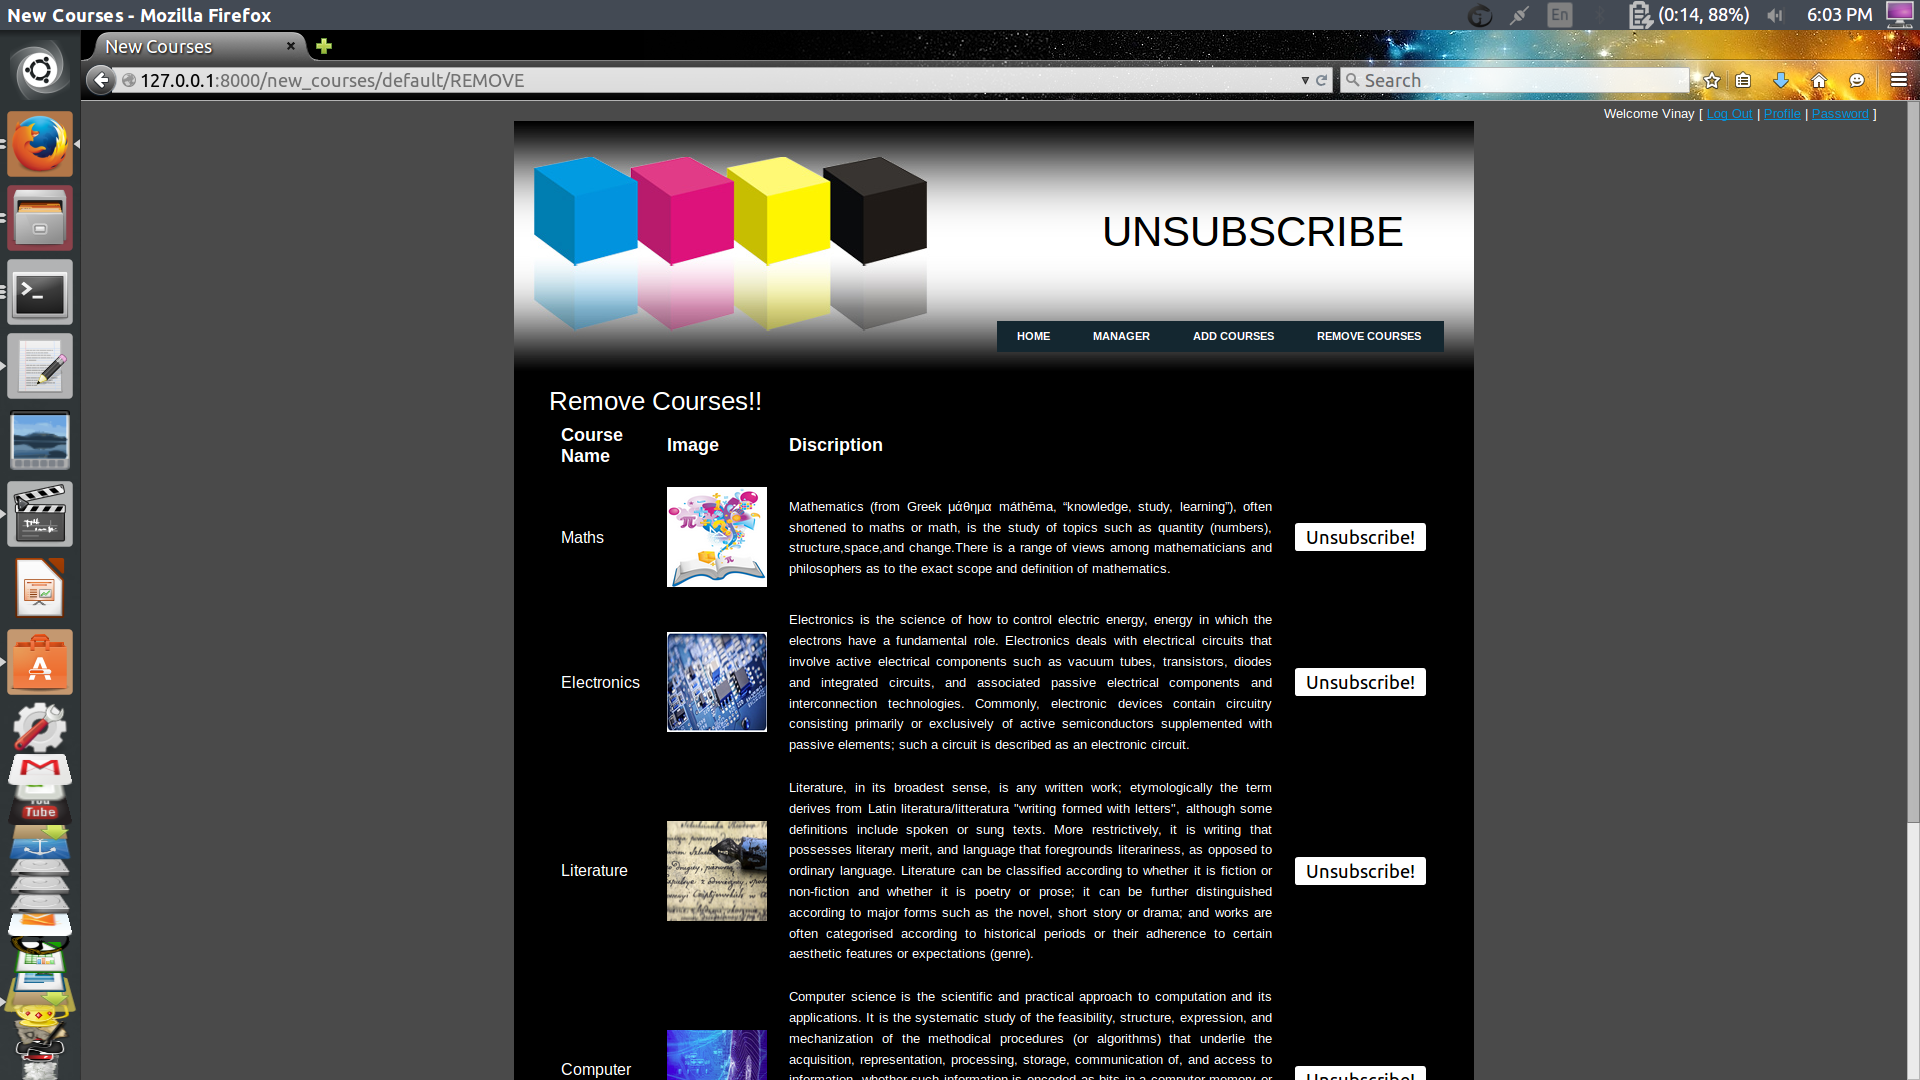
\includegraphics[width=110mm]{remove.png}
\caption{Remove course}
\end{figure}
\begin{figure}[ht!]
\centering
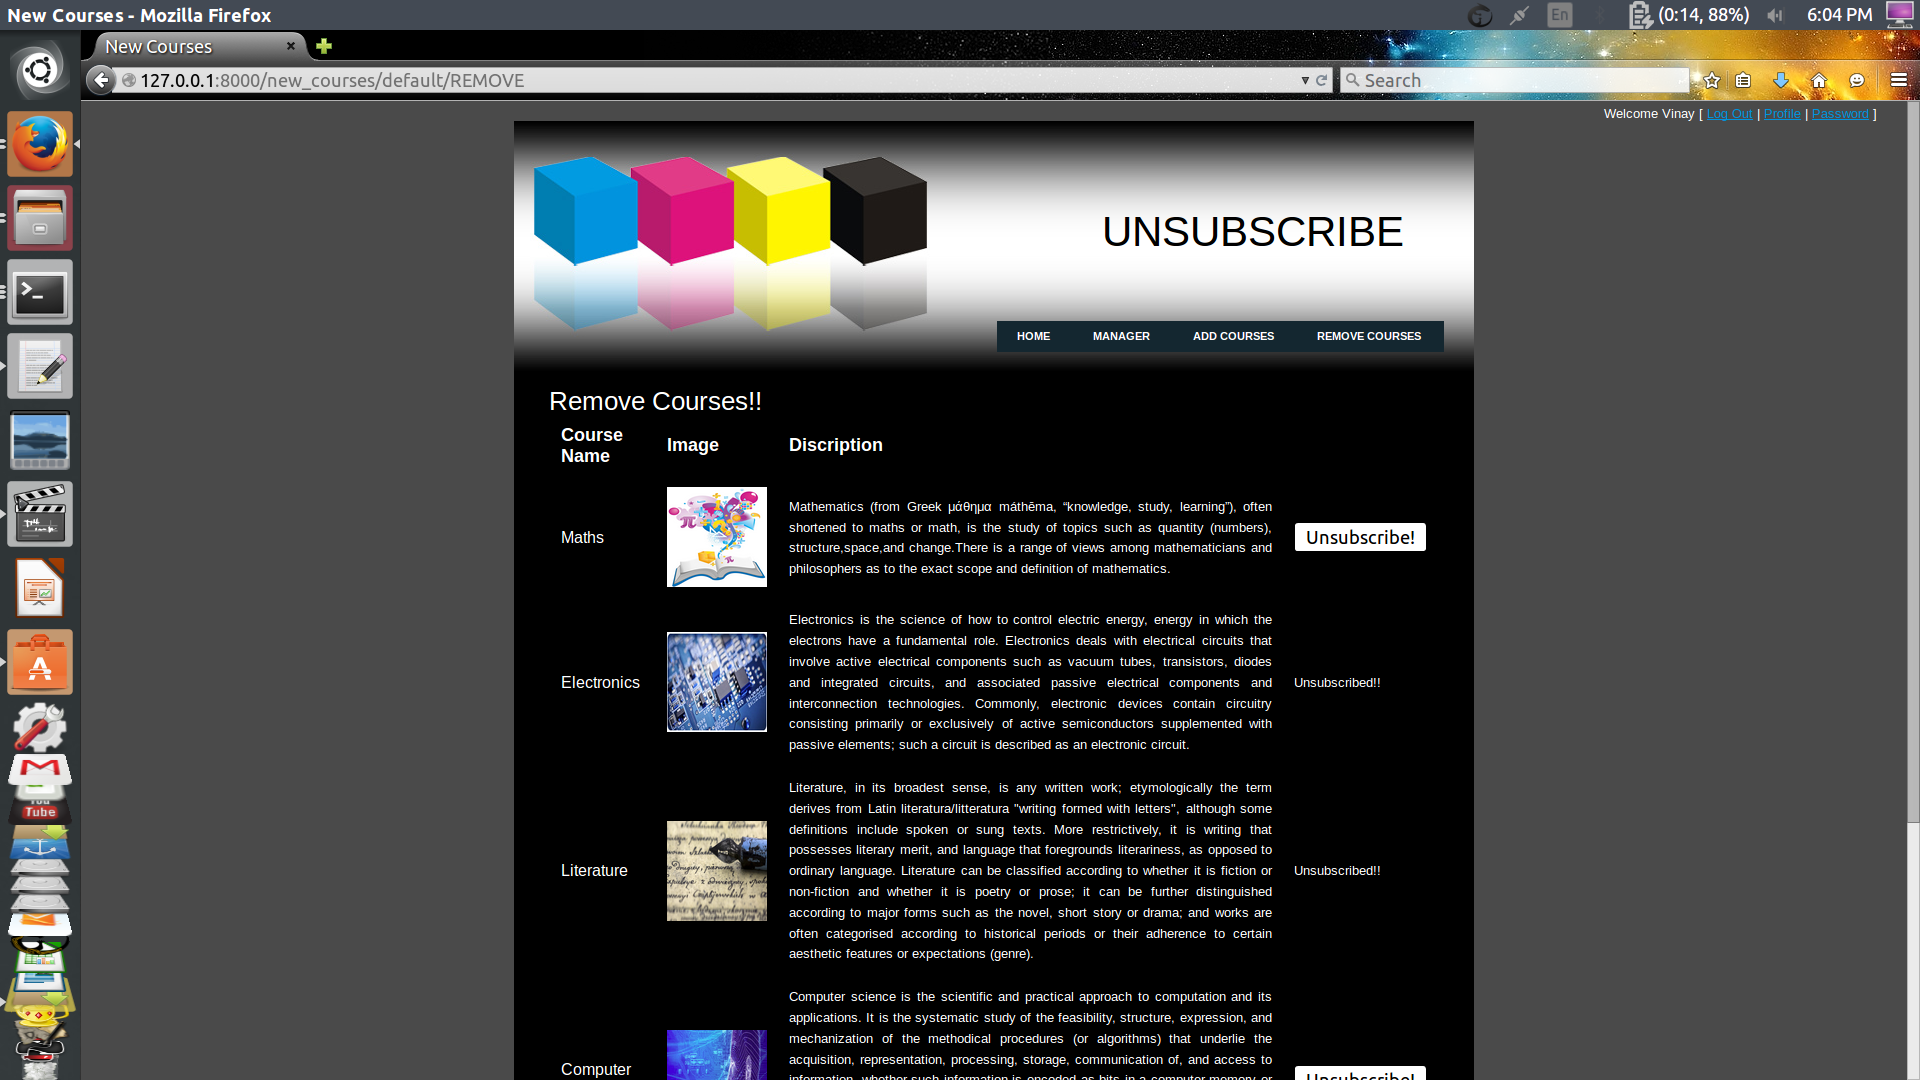
\includegraphics[width=110mm]{removed.png}
\caption{Removed course}
\end{figure}
\begin{figure}[ht!]
\centering
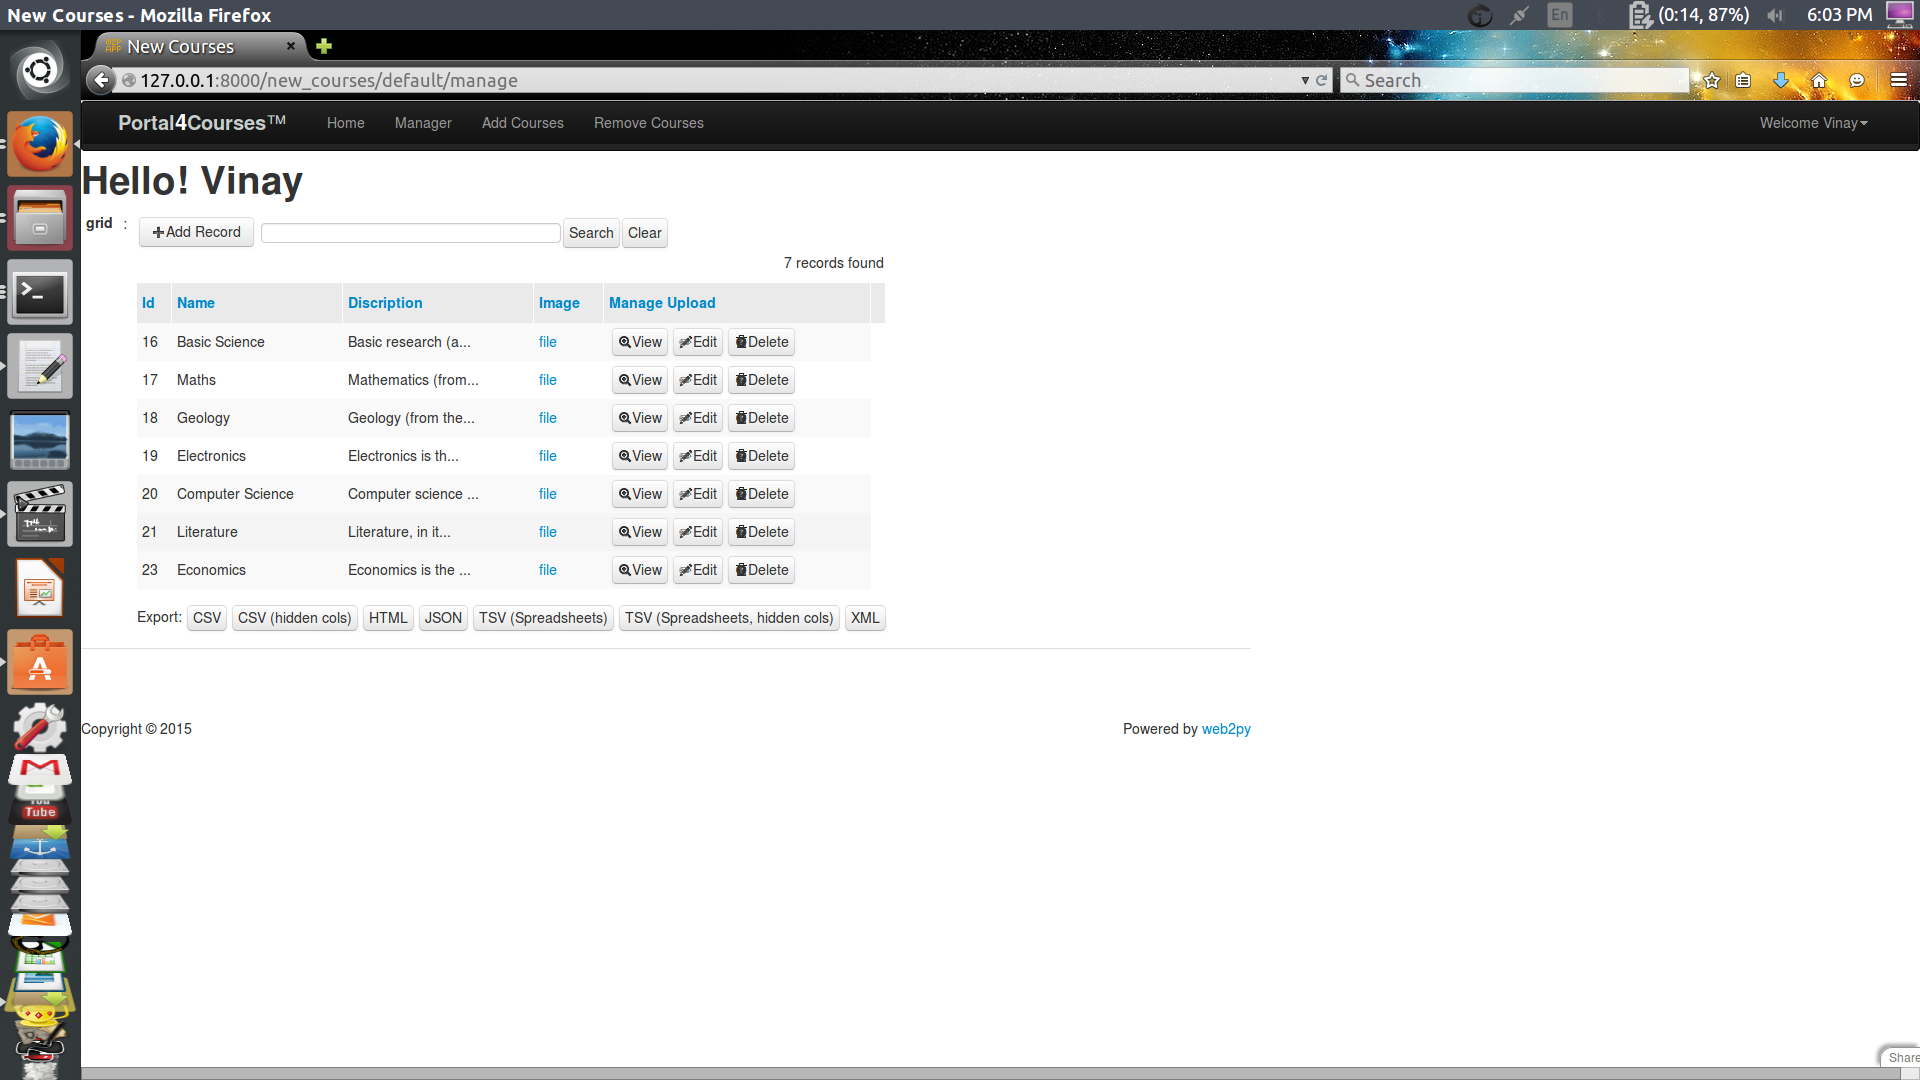
\includegraphics[width=110mm]{admin.png}
\caption{Adding new course to Database}
\end{figure}
\begin{figure}[ht!]
\centering
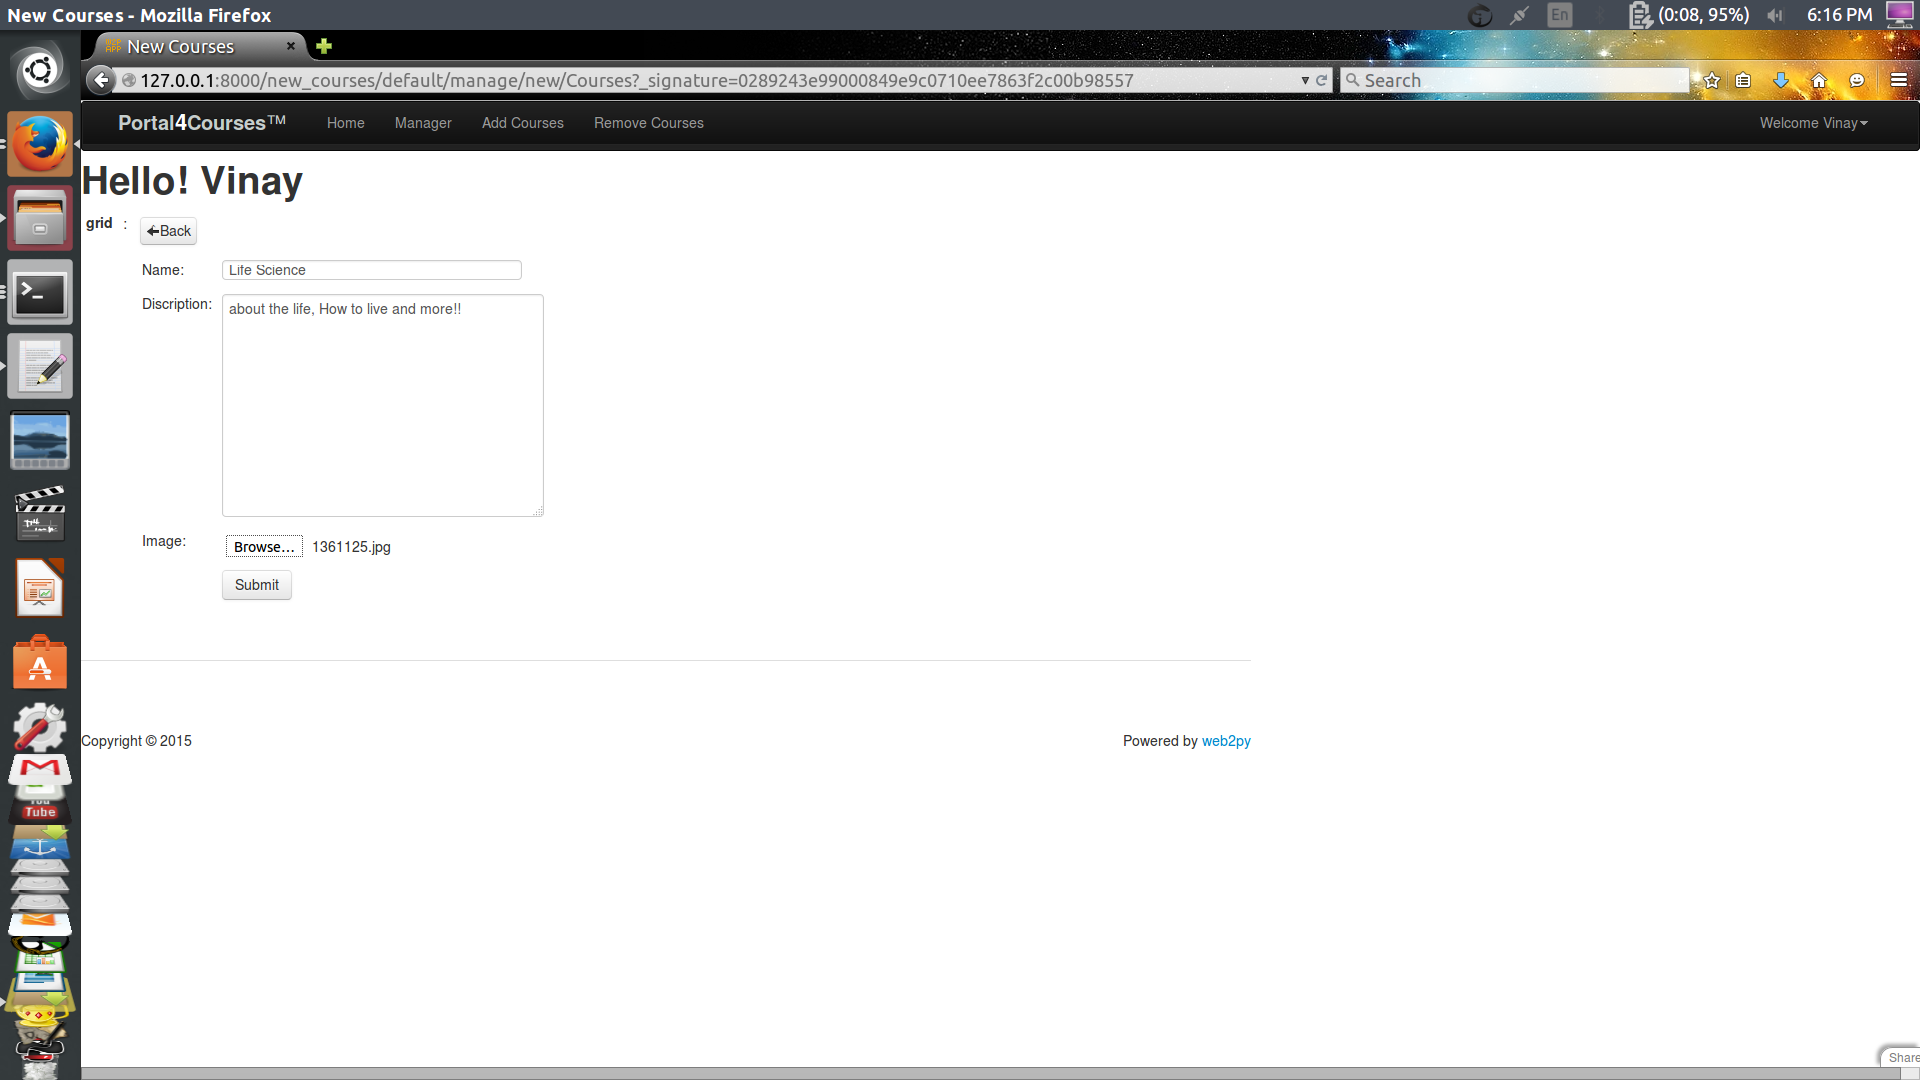
\includegraphics[width=110mm]{Add_new.png}
\caption{New course description}
\end{figure}
\begin{figure}[ht!]
\centering
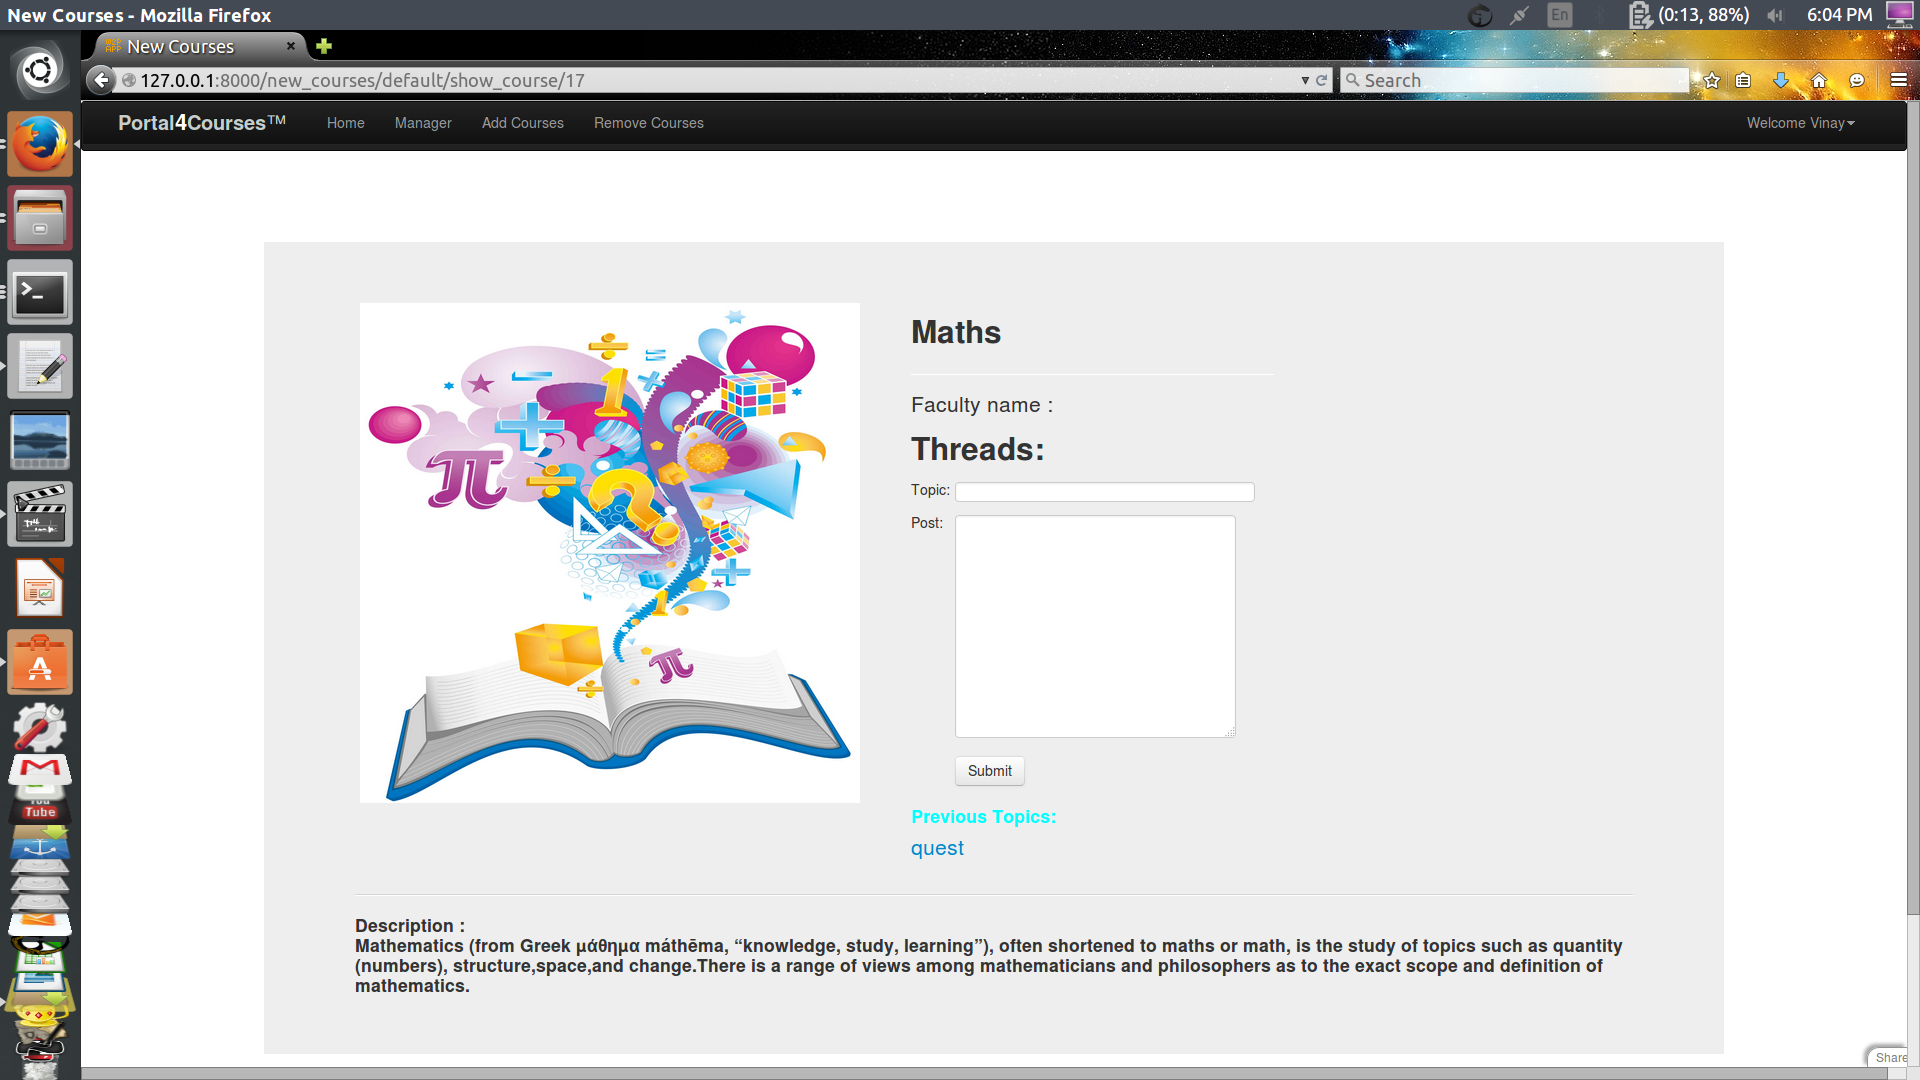
\includegraphics[width=110mm]{course.png}
\caption{One of the course}
\end{figure}
\begin{figure}[ht!]
\centering
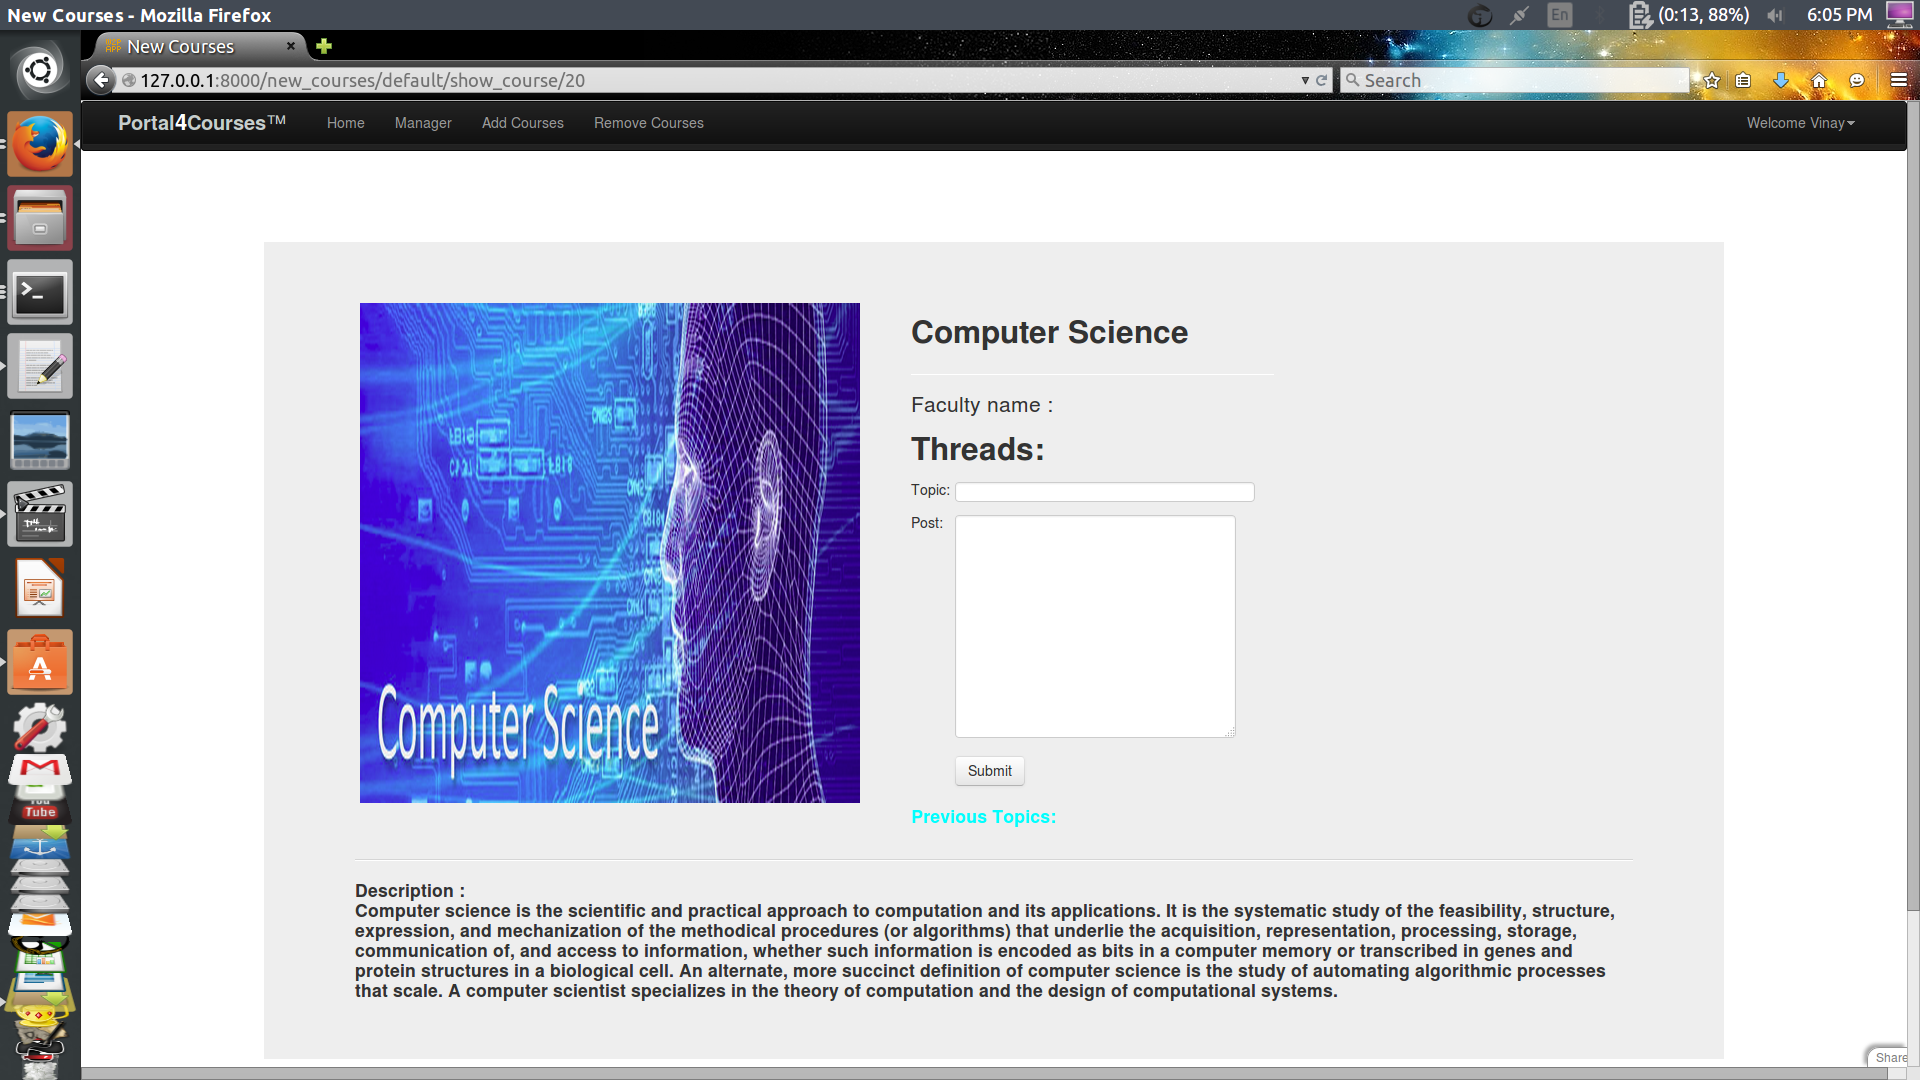
\includegraphics[width=110mm]{course1.png}
\caption{ Other Course}
\end{figure}
\begin{figure}[ht!]
\centering
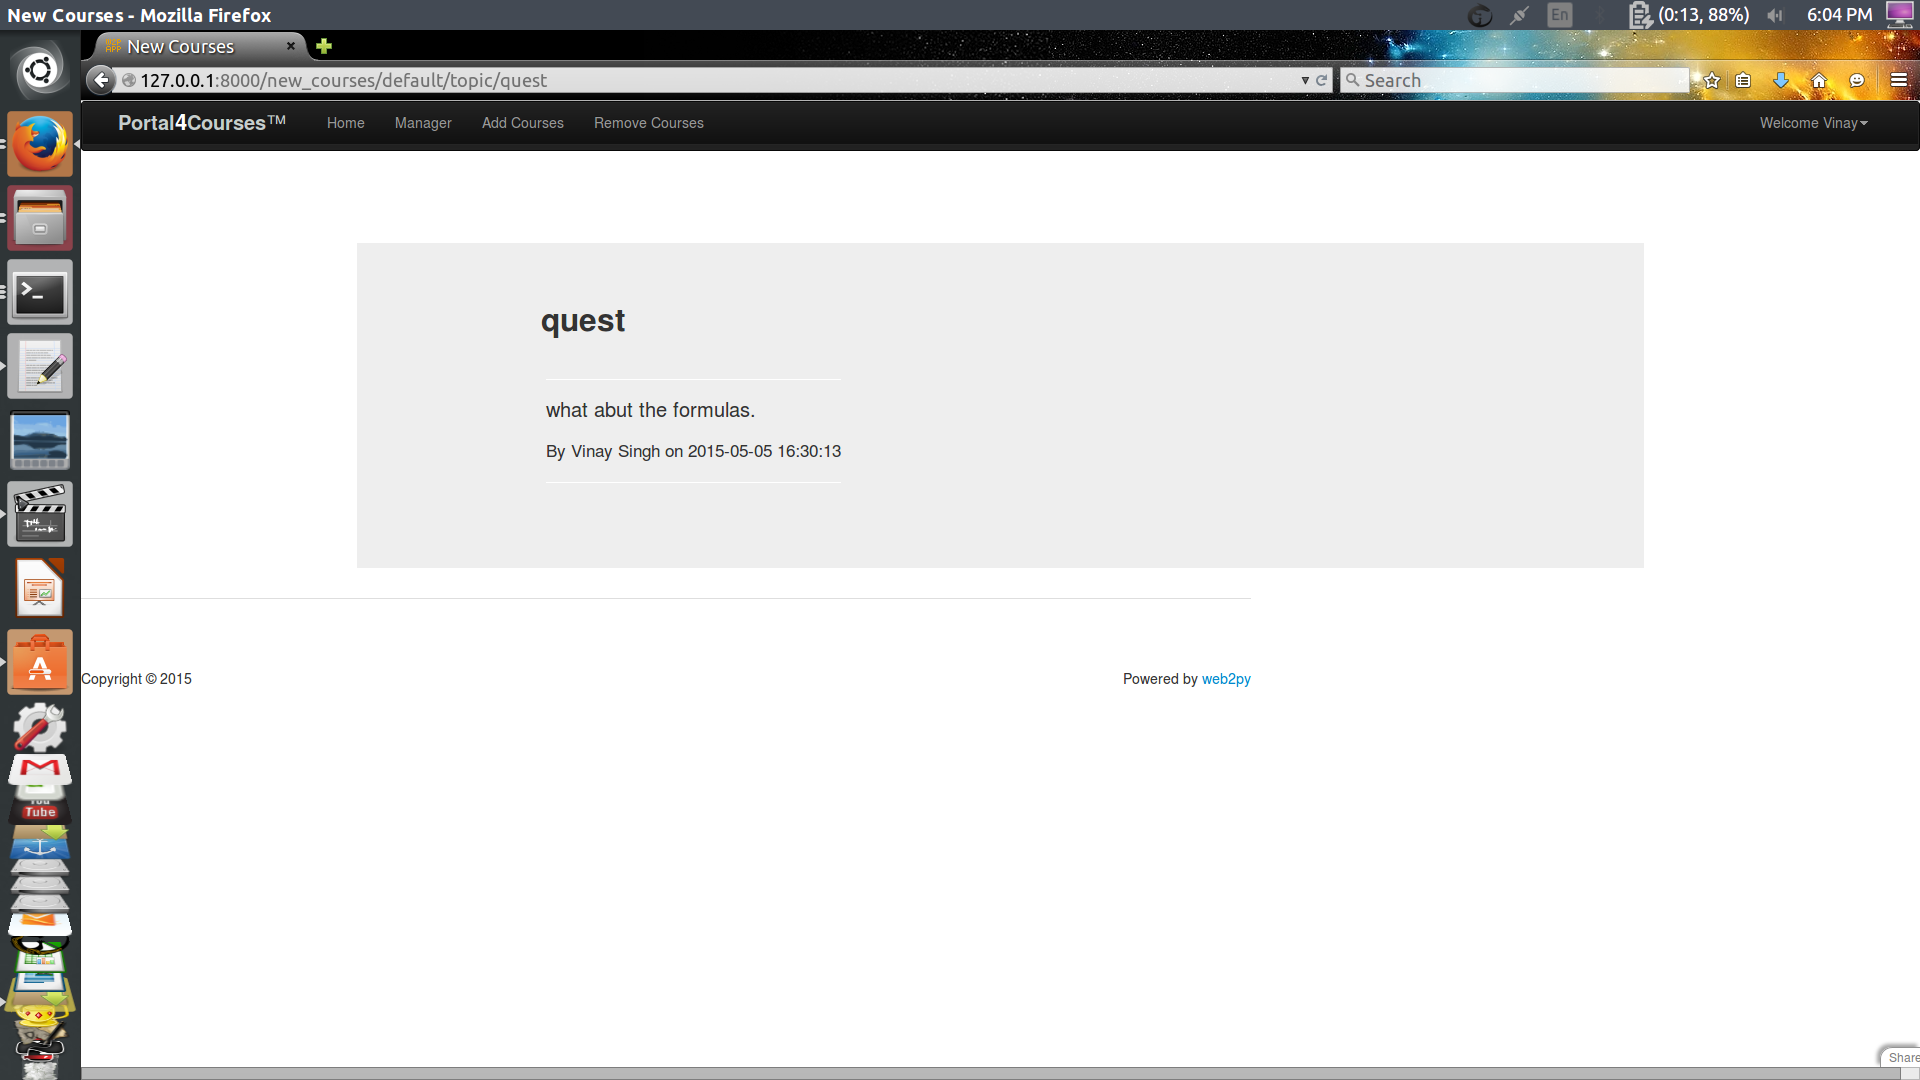
\includegraphics[width=110mm]{thread_post.png}
\caption{View the threads}
\end{figure}
\newpage
\end{document}
